\chapter{Plant Design} \label{chapProdPlantDesign}

This chapter and the following one address the design from scratch (i.e. greenfield) of a production node. Greenfield design is often a hard task since it involves risk, uncertainty and the definition of many assumptions which are hard to set since the production node only exists in our minds.\par

In general, this activity is complicated. Luckily, there are some general rules and framework that can help in this activity. When historical data from previous experience (or similar production nodes) are available, the data-driven approach helps to work with few but robust information. When historical data are not available, the definition of a kinematic/engineering model may help to get trustful estimates.\par

This chapter focuses on the problems related to the design of the plant:

\begin{enumerate}
    \item clustering items into product families;
    \item facility location;
    \item technology and asset choice;
    \item auxiliary systems design;
    \item definition of the number of assets;
    \item layout design.

\end{enumerate}

Chapter \ref{chapProdProcessDesign} focuses on the problems related to the design of the processes:

\begin{enumerate}
    \item Inventory policy design;
    \item Workstation design;
    \item Handling design.

\end{enumerate}

Figure \ref{fig_prod_plant_design} presents a cascade procedure, inspired to ~\cite{Heragu} showing these nine tasks for the design of a greenfield production node. This procedure is known in the literature as “facility design” and guides all the activity to transform a greenfield to a production plant.

% INSERT fig_prod_plant_design
\begin{figure}[hbt!]
\centering
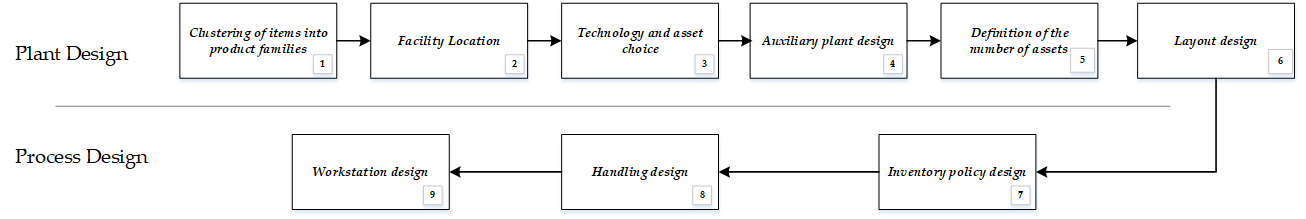
\includegraphics[width=1\textwidth]{sectionProduction/design_plant_figures/fig_prod_plant_design.png}
\captionsetup{type=figure}
\caption{Hierarchical framework for facility design.}
\label{fig_prod_plant_design}
\end{figure}



\section{Clustering parts into product families (P1)} \label{secClusteringParts}
Engineering is about complexity. Companies rely on engineers and engineering science since they are able to use tools and method to:

\begin{enumerate}
    \item pickup a complex problem;
    \item reduce its complexity;
    \item understand the problem;
    \item find a method to solve the problem;
    \item solve the problem.

\end{enumerate}

Production nodes are responsible for creating goods, i.e. parts $i$. Globalisation and mass customisation trends lead production nodes to incredibly high levels of complexity. This complexity is measurable in terms of:

\begin{itemize}
    \item The size of the product portfolio (i.e. the number of different parts $i$);
	\item The production volume $Q_{G,i}$ (i.e. the number of items produced by the plant $G$, for each type of part $i$).

\end{itemize}

These metrics are important to identify an adequate production technology, with a proper throughput $TH_j$ for each resource $j$; but this task can be hard when the number of parts $i$ is high (e.g. more than 1000). For this reason, it is good practice to cluster items into homogeneous families with similar features in order to reduce the complexity of the problem and focus on similar entities. According to Section \ref{secDecisionPatterns}, this is a version of the family problem, applied to a production system.

\subsection{Model-driven methods (D2)}

The design of a production system is all about creating an environment for a smooth and efficient production of goods. Empirically, the evidence shows that grouping parts $i$ with similar production cycle (i.e. route $e$) is an excellent way to improve efficiency. Model-driven approaches rely on the definition of an incidence matrix $X_{ij}$, defined as:

\begin{equation}
   \begin{split}
   X_{ij}=\left\{
                \begin{array}{ll}
                  1\ & if\ part\ i\ needs\ resource\ j\ in\ its\ production\ process\\
                  0 & otherwise\\
                \end{array}
              \right.
   \end{split}
\end{equation}

The diagonalisation of the matrix $X_{ij}$ into a matrix $X_{ij}^\delta$ is used to identify groups of homogeneous parts (see Figure \ref{fig_prod_matrix_diagonalisation}).

% INSERT fig_prod_matrix_diagonalisation
\begin{figure}[hbt!]
\centering
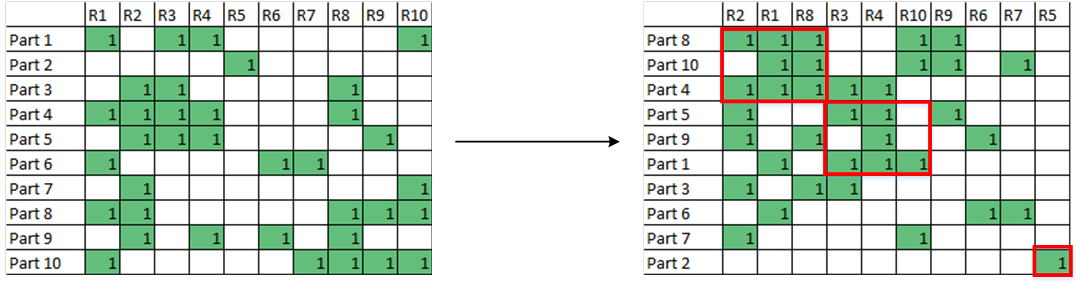
\includegraphics[width=1\textwidth]{sectionProduction/design_plant_figures/fig_prod_matrix_diagonalisation.png}
\captionsetup{type=figure}
\caption{Diagonalisation of a part-resource incidence matrix.}
\label{fig_prod_matrix_diagonalisation}
\end{figure}

Any diagonalisation algorithm is suitable to identify clusters of parts and resources since the model assumes that operations can be improved when the clusters of parts using the same subset of resources are handled together. For the sake of completeness, we mention the direct clustering algorithm ~\cite{Chan1982}, and the rank order clustering algorithm ~\cite{King1980} that produce the diagonalization of $X_{ij}$. \par

Once product families $\pi\in\Pi$ are defined, the rest of the design of the production node should consider the family $\pi$ instead of all the parts $i\in\pi$, so that the complexity due to the variety of the size of the product portfolio is reduced. In case, the number of families is still difficult to handle (e.g. higher than 100 families). A Pareto analysis  may help. For example, if a small subset of families (e.g. the 20\%) produces the major amount of the volumes $Q_{G,i}$, it is good to consider only the first 20\% of the families to reduce the complexity and the bias in the other design stages (see Figure \ref{fig_prod_pareto}).

% INSERT fig_prod_pareto
\begin{figure}[hbt!]
\centering
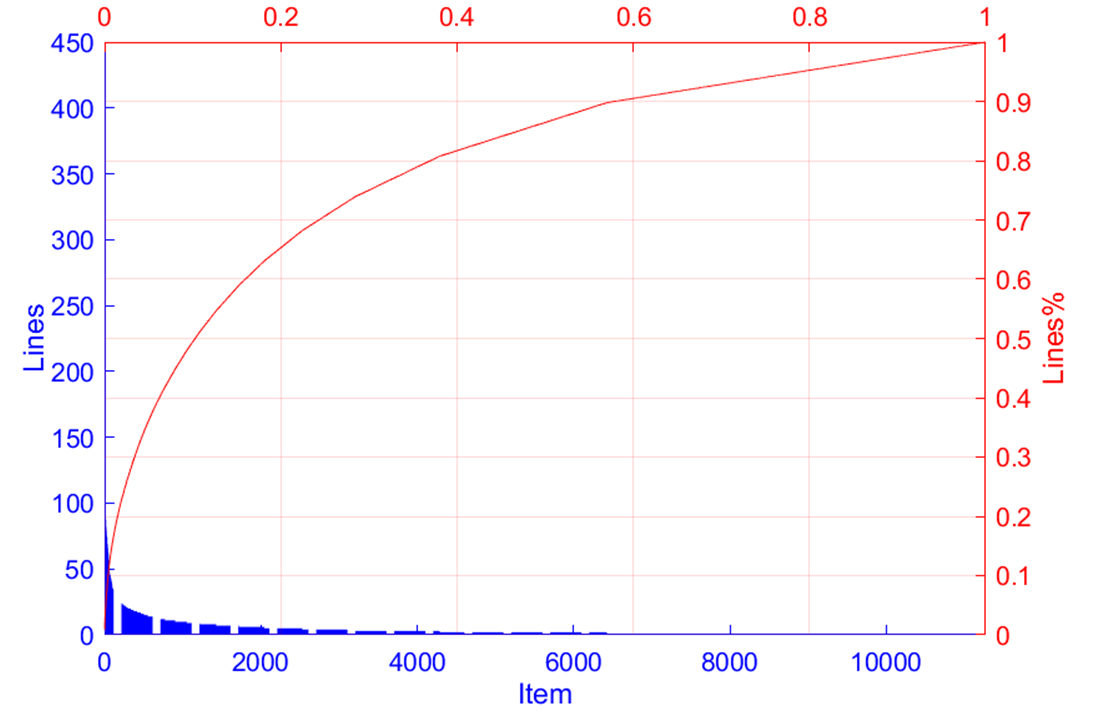
\includegraphics[width=0.9\textwidth]{sectionProduction/design_plant_figures/fig_prod_pareto.png}
\captionsetup{type=figure}
\caption{Pareto curve of a production plant where the first 40\% of the items produces the 80\% of the production volume (i.e. the number of production lines)}
\label{fig_prod_pareto}
\end{figure}

Clustering does not guarantee cluster are feasible in practice. For example, a cluster to be assigned to a group of machines may exceed the available working time of the resources. To solve this feasibility problem, an original capacitated clustering algorithm is proposed ~\cite{Tufano2020ISM}.  The algorithm is inspired to hierarchical clustering with a capacity constraint. Let $d_i$ be the \textit{demand} (e.g. the total working time) of a point (i.e. a part) $i$ and $C$ the maximum capacity of a cluster. The algorithm works similarly to algorithm \ref{algo_dist_CST}\footnote{The source code of Algorithm \ref{algo_dist_CST} is available \href{https://github.com/aletuf93/logproj/blob/master/logproj/ml_unsupervised_models.py}{here}}. The outcome of this algorithm is a set of clusters whose cardinality is unknown in advance. Each cluster $k$ has a total demand $d=\sum_{i\in k} d_i$, with $d\le C$.

\subsection{Data-driven methods (D1)}

The matrix $X_{ij}$ can be seen as the learning table introduced in chapter \ref{chapUnsupervisedLearning}. It consists of $n$ observations (one for each part $i=1,\ldots n$) and $p$ features (one for each resource $j=1,\ldots,p$). Data driven-methods enhance more powerful applications, by defining the similarity of the resources $j$, given the set of parts they can process. The incidence matrix $X_{ij}$ can, then, be transformed into a proximity matrix $D_{ik}$ (where $i$, and $k$ are both parts) by using a similarity index (see section \ref{secHierarchicalClustering}). Similarity indexes were born in the biological, and are defined using:

\begin{itemize}
    \item $a$, the number of resources processing by both $i$, and $k$;
	\item $b$, the number of resources processing only by $i$, and not by $k$;
	\item $c$, the number of resources processing only by $k$, and not by $i$;
	\item $d$, the number of resources processing neither by $i$, nor by $k$.

\end{itemize}

Using $a$, $b$, $c$ and $d$, the matrix $D_{ik}$ is defined for all the couples of resources $(i,k)$ using $d_{ik}=1$, where $s_{ik}$ is a similarity index. The most famous is the Jaccard index:

\begin{equation}
    s_{ik}=\frac{a}{a+b+c}
\end{equation}

For the sake of completeness, there are other many other definitions of similarity coefficients $s_{ij}$, as: the simple or relative matching coefficients ~\cite{Heltshe1988}, Yule coefficients, Rogers and Tanimoto coefficients ~\cite{Jackson1989}, Baroni-Urbani coefficients ~\cite{Buser1976}, Sorenson coefficient ~\cite{Yin2005}. Given $D_{ik}$, hierarchical clustering (see section \ref{secHierarchicalClustering}) is used to agglomerate parts into clusters.\par

The same procedure can be applied to create clusters of similar resources $j$ to locate close to each other on the plant layout. So far, the data-driven approach does not add too much to the classical model-driven approach.\par

There are unlucky but ordinary circumstances where the route $e$ of a product is unknown (e.g. not available in the information system during the planning). In this case, the data-driven approach is useful by combining different type of data to determine product families. There are many features that can enter the matrix $X_{ij}$, for example:

\begin{itemize}
    \item the set of processing resources $j$;
	\item the size of the part $i$;
	\item the volume and weight of $i$;
	\item the description of the item $i$;
	\item the package or the vehicle needed to transport $i$;
	\item the supplier of $i$;
	\item the customer of $i$;
	\item the bill of materials of $i$.

\end{itemize}

Given a matrix $X_{ij}$ with all the available information, it is necessary to investigate (e.g. using historical data) if a correlation exists between one of the features and the route $e$. If a correlation exists, feature selection should be performed, and unsupervised learning algorithms can be applied. Many unsupervised learning algorithms can be used as:

\begin{itemize}
    \item the k-means (see section \ref{secKmeans}), suitable when all the data are numerical and with the same unit of measure (e.g. length, height and width);
	\item the Gaussian mixture model (see section \ref{secGaussianMixture}), suitable when all the data are numerical and with the same unit of measure (e.g. length, height and width) and values are normally distributed within the same cluster;
	\item hierarchical clustering (see section \ref{secHierarchicalClustering}), when data are categorical or provided by a binary incidence matrix $X_{ij}$ or a proximity matrix $D_{ik}$.

\end{itemize}

Measuring the goodness of a cluster is a hard task both using a data-driven and a model-driven approach. The underlying assumption is that when clusters are homogeneous, the $WIP_j$ of the resources is minimised since flows are smooth. In addition, if resources processing the same product family are placed close to each other, the $LT_e$ is reduced and provides a higher $LoS_e$.


\section{Facility location (P6)} \label{secFacilityLocationProd}
Facility location problem regards the definition of an adequate location (i.e. latitude and longitude) to place a production node. The production plant should be placed within an area where the costs are minimised. This type of decision is highly prescriptive and guided by engineering models since it is difficult to collect data on the previous realisation of this choice.

\subsection{Model-driven methods (PS4)}
The main underlying assumption of these models is that a plant should be placed such that the costs linked with its location are minimised. Some other crucial aspects connected with the facility location are:

\begin{itemize}
    \item the cost of the direct labour of a location;
    \item the cost of the energy;
    \item the cost of the land and the building;
    \item the connection to distribution networks (e.g. rail/water)
    \item the availability of raw materials (e.g. sand)
    \item the transportation costs.

\end{itemize}

This problem can be solved using optimisation when all this information is available for any alternative. When alternative locations are close to each other, transportation cost may be the only significant variable to take into account (and to minimise) in the definition of the facility location.\par

In this case, the problem can be solved by using a kinematic model based on the minimisation of the travelled distance. Let $S$, with $s\in S, s=1,...,k$ be the set of customers and suppliers of the production plant to place. Each point $s$ is characterised by its longitude and latitude ($lon_s$,$lat_s$), and an estimate of the number of trips $w_s$ travelled between the production node and $s$. To find the point minimising the distance, it is necessary to transform the longitude and the latitude into cartesian coordinates. There are many methods allowing to do that. Here the Mercator projection ~\cite{Snyder1978} is used, where:

\begin{equation}
    x_s=R\times lon_s^{RAD}
    \label{eq_mercator_x}
\end{equation}

\begin{equation}
    y_s=R\times\ln{\left[\left(\frac{1-e\times\sin{\left(lat_s^{RAD}\right)}}{1+e\times\sin{\left(lat_s^{RAD}\right)}}\right)^\frac{e}{2}\times t g\left(\frac{\pi}{4}+\frac{lat_s^{RAD}}{2}\right)\right]}
    \label{eq_mercator_y}
\end{equation}

Where $lon_s^{RAD}$ and $lat_s^{RAD}$ are the coordinates using radians, $R=6378.14$ km is the equatorial radius, $e=0.0167$ is the eccentricity of the Earth. Given $x_s$ and $y_s$ for all $s\in S$, the problem is to find the coordinates $(x,y)$ to place the production plant, minimising:

\begin{equation}
    z=\min{\left\{d\left[\left(x,y\right),\left(x_s,y_s\right)\right]\times w_s\ \right\}}
\end{equation}

Where $d$ is an arbitrary distance function, for example:

\begin{itemize}
    \item Rectangular (or city block) distance: $\left|x-x_s\right|+\left|y-y_s\right|$;
	\item Euclidean distance: $\sqrt{\left(x-x_s\right)^2+\left(y-y_s\right)^2}$;
	item Squared Euclidean (or gravity) distance: $\left(x-x_s\right)^2+\left(y-y_s\right)^2$.

\end{itemize}

The mathematical minimum can be found by minimising $z$ ~\cite{Wesolowsky1972}. Nevertheless, it is almost impossible that this point coincides with a feasible physical location for the plant. For this reason, a gradient approach results much more useful to support the decision-maker. Let define a set $\Phi={(x_f,y_f)}$ containing the coordinates (using equations (\ref{eq_mercator_x}) and (\ref{eq_mercator_y})) of a number of available locations $f$. By considering a broader geofence, containing all the points in $\Phi$ and defining the value of $z$ for any point within the geofence, the gradient of $z$ can be identified. This way, the decision-maker could identify which direction is better to find an area for the new production plant. Many alternative procedures to minimise $z$ depending on $d$ can be found in ~\cite{Salhi1996}.\par

Nowadays, due to the variability of the market demand and the shortness of the duration of the contract, the reliability of a static approach to solving the facility location problem may be reduced. As well as with time series, which considers the evolution of an event over time, by repeating the calculation of the optimal location with different time horizon it is possible to define optimal location using a probabilistic approach. Let $z^\ast$ be the set of optimal locations $(x_t^\ast,y_t^\ast)$ calculated on a time horizon $T$, where $t\in T$. Then, the minimum of the function:

\begin{equation}
    z^\pi=\min{\left\{\sum_{t\in T} d\left[\left(x,y\right),\left(x_t^\ast,y_t^\ast\right)\right]\right\}}
\end{equation}

Identifies the optimal location over a time horizon $T$\footnote{The package logproj provides method to deal with facility location problems \href{https://github.com/aletuf93/logproj/blob/master/logproj/P6_placementProblem/facility_location_definition.py}{here}}.

\section{Auxiliary systems design (P4)}
Auxiliary systems are any technological asset that does not directly add value to the finished product, but it is necessary to perform tasks. Examples of the auxiliary systems are:

\begin{itemize}
    \item the lighting systems of the production site;
    \item the air conditioning system (i.e. heating and cooling);
    \item the systems for the production of energy (e.g. electricity/steam),
    \item the systems for the production of other technological fluids (e.g. compressed air);
    \item the systems for the reduction of the noise.

\end{itemize}

All of these systems involve precise prescriptive design models based on engineering models. These models cannot be validated before the realisation of the system that is usually costly. For this reason, the whole design phase relies on engineering procedure based on indices and coefficient belonging to different knowledge domains that are not deeply analysed in this work ~\cite{Colombo2012}.

\section{Technology and asset choice (P2)} \label{secTechChoiceProd}
This activity involves the determination of the proper technologies and level of automation to perform production tasks. This is a technology assignment problem  since, given the features of the products and the demand, it is necessary to identify the throughput $TH_j$ for each resource and the lead times $LT_e$ associated with the production cycles. Depending on the level of automation and flexibility, it is possible to identify different production, layout and automation paradigms (see Figure \ref{fig_prod_flexauto1}) ~\cite{Groover2015}.


% INSERT fig_prod_flexauto1
\begin{figure}[hbt!]
\centering
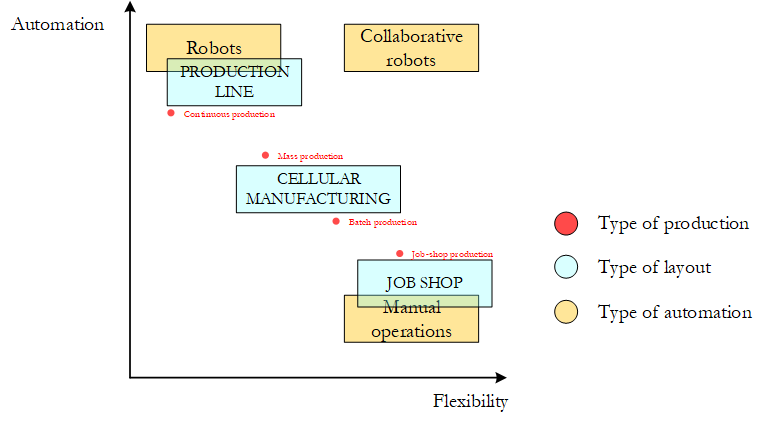
\includegraphics[width=1.0\textwidth]{sectionProduction/design_plant_figures/fig_prod_flexauto1.png}
\captionsetup{type=figure}
\caption{Flexibility-automation matrix for technology choice.}
\label{fig_prod_flexauto1}
\end{figure}

Three main layout configurations are identified:

\begin{enumerate}
    \item the production line: all the resources necessary to transform raw materials into a finished product are placed in line.
    \item cellular manufacturing: all the resources necessary to transform raw materials into a limited set of finished products are placed together. There is the possibility some tasks need resources outside the cell.
    \item resources are organised per type (milling machines, lathing machines, pressing machines).

\end{enumerate}

There are four production paradigms connected to these layout configurations:

\begin{itemize}
    \item continuous production: the production flow is continuous, with a fixed cycle time;
    \item mass production: the production flow is fast but not continuous since it requires small customisations (e.g. form-postponement, different labelling) in the end-of-line;
    \item batch production: the production flow has major interruptions due to the setup of machines (e.g. to change the die of a press);
    \item job-shop production: the production flow is slow and fragmented among the different departments.

\end{itemize}

The type of automation is different as well, since:

\begin{itemize}
    \item fully automated production line works with robots allowing high accuracy and modest cycle time, but with no flexibility to readapt the production;
    \item collaborative robots may work together with human operators in many applications (e.g. assembly lines) enhancing both the power of the automation and the flexibility of the manual operations;
    \item manual operations have the highest degree of flexibility, but with limited cycle time and a significant probability of errors.

\end{itemize}

The decision-maker should choose the possibilities that maximise the profit of the company within a pre-defined time horizon. In particular, it is important to have reliable forecasts on the workload and information on the investment cost for different technologies.

\subsection{Model-driven methods (PS3)}
Model-driven methods consider two metrics (already seen in section \ref{secClusteringParts}) to identify an adequate technological configuration:

\begin{itemize}
    \item the size of the product portfolio (i.e. the number of different parts $i$);
	\item the production volume $Q_{G,i}$ (i.e. the number of items produced by the plant $G$, for each type of part $i$).

\end{itemize}

By performing a Pareto analysis on the production volume for each part (see Figure \ref{fig_prod_flexauto2}):

\begin{itemize}
    \item few parts with high production volumes should be assigned to production lines;
    \item the majority of parts with extremely low volumes should be processed in the departments of a flow shop;
    \item cellular manufacturing, flexible manufacturing systems (FMS) and reconfigurable manufacturing systems (RMS) should be considered for parts with an intermediate behaviour.

\end{itemize}

% INSERT fig_prod_flexauto2
\begin{figure}[hbt!]
\centering
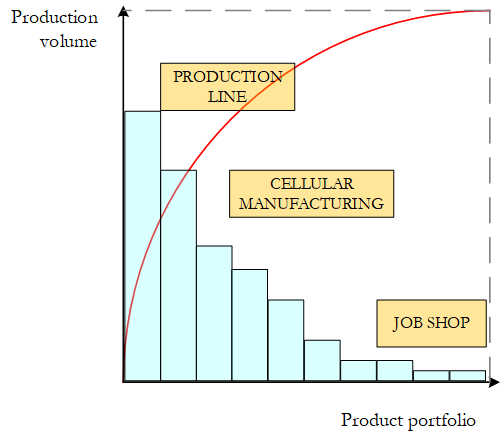
\includegraphics[width=0.8\textwidth]{sectionProduction/design_plant_figures/fig_prod_flexauto2.png}
\captionsetup{type=figure}
\caption{Classification of parts for technology and asset choice.}
\label{fig_prod_flexauto2}
\end{figure}

For each product, it is possible to identify the decoupling production volume $TH_i$ (part/hours) corresponding to an economic convenience between a production line and a job-shop production ~\cite{Pareschi2007}. Let the saturation of a resource $j$ be:

\begin{equation}
    U_j\left(TH_i\right)=\frac{THi\times t_j}{n_j\left(TH_i\right)\times3600}
\end{equation}

Where $TH_i$ is the production throughput (parts/hours), $t_j$ is the processing time per part (sec/part), $n_j(TH_i)$ the number of resources of type $j$, necessary to reach a throughput $TH_i$, 3600 is the number of available seconds per hour of resource $j$.\par

Considering a target saturation $K$ for a production line (e.g. the 90\%), the decoupling production volume for a part $i$ is $TH_i:U(TH_i)>K$, where:

\begin{equation}
    U(TH_i)=\frac{\sum_{j}{U_j\times n_j(TH_i)}}{\sum_{j}{n_j(TH_i)}}
\end{equation}

Resources $j$ are usually some tens. When they have a very different investment cost $C_J$ between each other, it is recommended to take into account this cost by setting:

\begin{equation}
    U(TH_i)=\frac{\sum_{j}{U_j\times{C_j\times n}_j(TH_i)}}{\sum_{j}{C_J\times n_j(TH_i)}}
\end{equation}

Once the function $U(TH_i)$ is defined, the decision between production line or job-shop should be made by setting $TH_i$ equal to the demand takt-time. If $U\left(TH_i\right)>K$, then there are good reasons to take into account the design of a production line. Otherwise, other layout models (cellular manufacturing or job-shop) should be considered.

\subsection{Data-driven methods (PS2)}

The choice of the production technology and the assets can be seen as an assignment problem where parts $i$ need to be assigned to an adequate technology. Observations of parts belonging to different production models help to identify the proper cluster. Classification models (see chapter \ref{chapLinearClassification}) can be used for the definition of the decision boundaries between the clusters. Figure \ref{fig_prod_flexauto3} illustrates a scatterplot identifying three different production technology. Blue dots are processed within the departments of a job-shop system. Red dots are products realised by machines organizes ad production cells and flexible manufacturing systems (FMS). Green dots are processed on manual workbenches able to perform any production task for any type of product.

% INSERT fig_prod_flexauto3
\begin{figure}[hbt!]
\centering
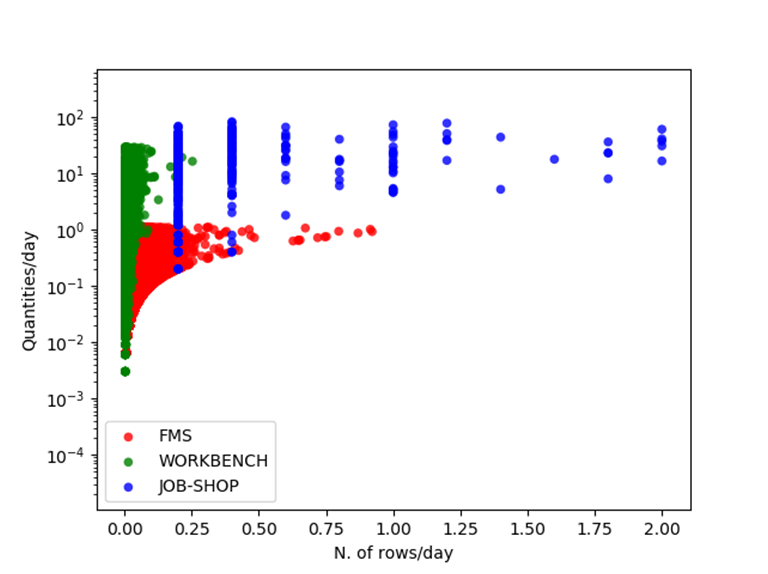
\includegraphics[width=0.9\textwidth]{sectionProduction/design_plant_figures/fig_prod_flexauto3.png}
\captionsetup{type=figure}
\caption{Classification of parts using the number of orders and the number of produces quantities per day.}
\label{fig_prod_flexauto3}
\end{figure}

The definition of such clusters within the same production node allows to immediately identify which layout configuration results suitable the most in case of re-design. In addition, the design of a classification model (see sectio \ref{chapLinearClassification}), can help to design the production flow of new products depending on the expectation of their market demand (i.e. the number of rows and the order quantity).

\section{Definition of the number of assets (P5)}
The definition of the number of assets identifies the power (i.e. the capacity) and the saturation of the resources. The utilisation $U_j$ must be as higher as possible for economic reasons, while the capacity $C_j$ should be enough to satisfy the market demand. Both these metrics impact the level of service since capacity act as a buffer (higher capacity allow for processing a production volume within a shorter time). As many power problems in other engineering disciplines, this problem is prescriptive and lead by an engineering model.

\subsection{Model-driven methods (PS4)}
Models to define the number of assets can be static or dynamic. When no information about the time is available, a static model should be chosen. Static models always work by considering:
\begin{itemize}
    \item $a_j$, the amount of time a resource $j$ is available over a time span (e.g. hours/day);
	\item $b_j$, the expected amount of working time required by the parts $i$ that need to be processed on $j$ (e.g. hours/day).

\end{itemize}

The minimum number of assets of type $j$ can be statically calculated as:

\begin{equation}
    n_j=\left\lceil\frac{b_j}{a_j}\right\rceil
\end{equation}

When the decision-maker has time-based information as:
\begin{itemize}
    \item the probability distribution $f_i(t)$ of the arrival of parts for each resource $j$;
	\item the probability distribution $g_{ij}(t)$ of the working time of each resource $j$.

\end{itemize}

A simulation approach can be used to identify the number of resources virtually. Simulation is a complex task performed on commercial simulation software. Each resource is associated with a queue where parts $i$ are placed when the resource is busy. By randomly generating parts $i$ and processing time (from $f$, and $g$) operations are virtualised, and the number of items waiting in queue is estimated. $U_j$, $C_j$ and $LoS_e$ can be estimated as well by iterating instances of the simulation. The probability distributions of the KPIs and the queue size suggest the decision-maker if the number of assets in the simulated configuration is appropriate or should be modified. By running different scenarios with a different number of assets, a satisfying configuration can be obtained. 

\section{Layout design (P6)} \label{secProdLayoutDesign}
The layout design is a placement problem involving the definition of the location on the plant layout for each resource $j$. It is a combinatorial problem, usually solvable by a model-driven approach using optimisation.

\subsection{Model-driven methods (PS1)}
The combinatorial problem can be modelled using the quadratic assignment problem as follows. Table \ref{tab_QAP} identifies the parameters of the problem.

% INSERT tab_QAP
\begin{figure}[hbt!]
\centering
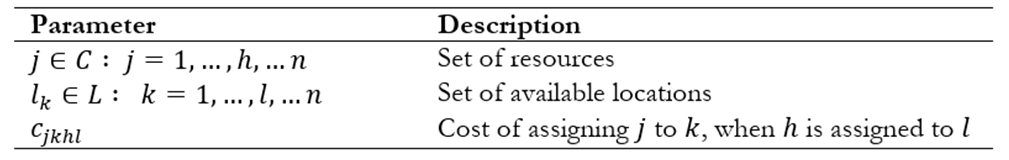
\includegraphics[width=0.9\textwidth]{sectionProduction/design_plant_figures/tab_QAP.png}
\captionsetup{type=figure}
\caption{Parameters of the quadratic assignment problem.}
\label{tab_QAP}
\end{figure}

The model is as follows.

\begin{equation}
   \begin{split}
   X_{jk}=\left\{
                \begin{array}{ll}
                  1\ & if j assigned to k process\\
                  0 & otherwise\\
                \end{array}
              \right.
   \end{split}
\end{equation}

\begin{equation}
    \begin{split}
        \min{\sum_{j\in C\ }\sum_{k\in L}\sum_{h\in C}\sum_{l\in L}{c_{jkhl}\ x_{jk}\ x_{hl}}}\\
        \sum_{j\in C}{x_{jk}=1\ , k=1,\ldots,n}\\
        \sum_{k\in L}{x_{jk}=1\ , j=1,\ldots,n}\\
        x_{jk}\ integer\\
    \end{split}
\end{equation}

By setting $c_{jkhl}$ equal to the distance between control points $k$, and $l$, times the number of trips exchanged between resources $j$, and $h$, the problem consists in finding the layout configuration which minimises the total travelled distance. Unfortunately, the problem is quadratic and a solver may take forever to find the configuration of decision variables $x_{jk}$ corresponding to the minimum solution value. For this reason, a number of suboptimal algorithms are introduced to find adequate configuration (without the warranty of optimality). These algorithms are organized into:

\begin{itemize}
    \item construction algorithms, to find a feasible solution starting from the input data;
    \item local search algorithms, to improve an existing feasible solution.

\end{itemize}

\subsubsection{Construction algorithms}
Construction algorithms split the problem of the layout configuration into two different subproblems:

\begin{enumerate}
    \item control points ranking;
    \item control points placement.

\end{enumerate}

Relevant methods are the total-closeness-rating, the ALDEP ~\cite{Rosenblatt1979}, the CORELAP ~\cite{Adendorff1972} and the relationship diagramming method ~\cite{Plotnick2007}. All of these have a ranking and a placement procedure.

\subsubsection{Local search algorithms}
The solution produced by a construction algorithm may be far from optimality. For this reason, local search algorithms perform \textit{moves} (i.e. little modification of the incumbent solution) to improve the solution value.\par

Local search algorithms are the 2-opt, 3-opt exchange ~\cite{Potvin1989} and CRAFT ~\cite{Scriabin1985}. The 2-opt and 3-opt are general-purpose local search methods that make exchanges between groups of 2 or 3 elements.

Regardless of the methodology used to solve the plant layout problem, a graph $G\left(V,A\right)$ of the system can be defined and visually investigated to identify criticalities. The flows exchanged between control points can be aggregated by arcs or nodes and represented by projecting $G$ on the plant layout (see Figure \ref{prod_layout_visual})\footnote{The source code to deal with the representation of a from-to matrix is available \href{https://github.com/aletuf93/logproj/blob/master/logproj/P3_flowProblem/assessFlows.py}{here}.}.

% INSERT prod_layout_visual
\begin{figure}[hbt!]
\centering
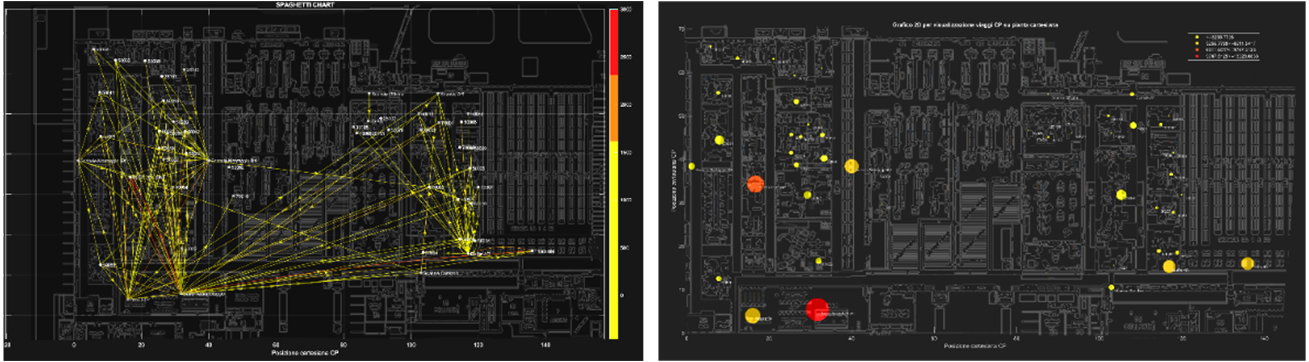
\includegraphics[width=0.9\textwidth]{sectionProduction/design_plant_figures/prod_layout_visual.png}
\captionsetup{type=figure}
\caption{Visual representation of the material flows aggregated by arcs (on the left) and by nodes (on the right).}
\label{prod_layout_visual}
\end{figure}

\section{Applications}
This section illustrates two applications of plant and process design within two different industrial sectors (food and automotive). The aim is to show the generalisation of the methods proposed in the previous chapters, and the effect of the data-driven methods in applied design case studies. In particular, the first case study is mainly model-driven, while the second is more data-driven.

\subsection{Plant Design of a food catering plant} \label{secCateringDesign}

This section applies the methodology to design a food catering plant from scratch. The food catering industry is responsible for supplying warm, safe, and tasty food to schools, hospitals, and nurseries, as well as to company canteens. The production plant of a food catering industry is known as a \textit{centralised kitchen} (CEKI).\par

Typically, a middle-size CEKI can prepare, pack, and deliver more than 10.000 meals per day by working in a short-spanned time batch (e.g., from 5.00 AM to 11.30 AM for the lunch service); it provides food service within a short-range, usually at distances under 30 km. The type of service is also characterized by the temperature at which the meals are distributed. Three alternative temperature profiles are possible:  

\begin{itemize}
    \item cook-warm: the product is cooked and maintained warm (above 65 \degree C) until it is consumed; 
    \item cook-chill: the product is cooked, blasted, and delivered to the customer who re-warm it before service ~\cite{Williams1996};
    \item cook-chill-re-warm: this is when cook-and-chill products are rewarmed at the CEKI and delivered according to the cook-warm profile.
\end{itemize}

Among these profiles, cook-warm is the most critical for safety issues because the product’s temperature must be maintained above the danger zone (4–65 \degree C) at which bacteria propagate exponentially ~\cite{Rahman2002}. The cook-warm meals should be conserved at conditions that are outside the danger temperature range to comply with safety rules and standards from the time they are produced until their consumption and should be necessarily subjected to continuous and expensive hazard analyses and critical control points (HACCP), as well as monitoring and control of the processing tasks. \par

A CEKI can implement all these three production temperature profiles leading to a more complex organisation of the operations. The assessment of the current production environment is a fundamental step to properly design a new plant. This procedure has already been illustrated in \ref{secFoodCateringControl}.

\subsubsection{Clustering products into families}
For analysing the extant production mix, the previous product families are considered. Product families are based on the commercial class to which a product belongs. Different families are defined for the components of a menu (e.g. main dish, side dish, fruit, dessert, vegetables, mineral water). Figure \ref{fig_prod_CAMST_productFamilies} illustrates the relative importance of each product family by using a Pareto analysis.


% INSERT fig_prod_CAMST_productFamilies
\begin{figure}[hbt!]
\centering
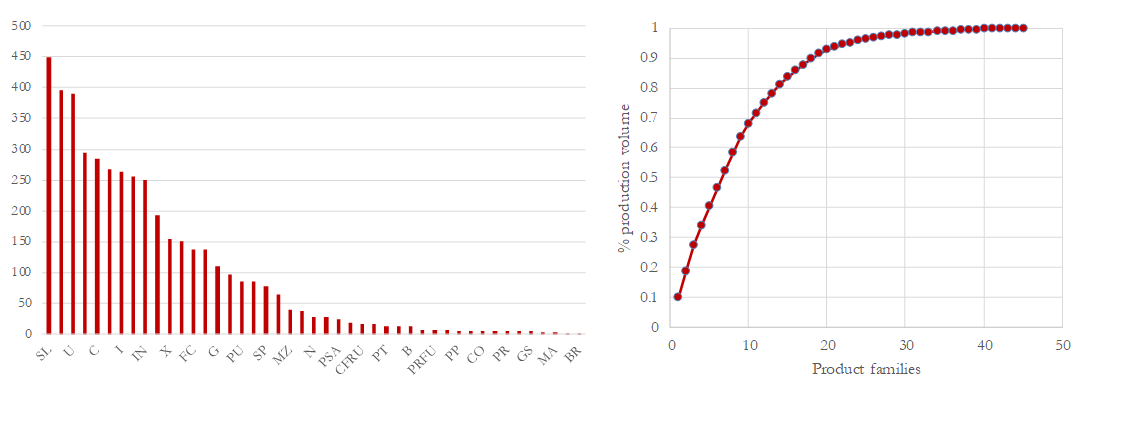
\includegraphics[width=0.9\textwidth]{sectionProduction/design_plant_figures/fig_prod_CAMST_productFamilies.png}
\captionsetup{type=figure}
\caption{Histogram and Pareto chart of the product volumes within each product family.}
\label{fig_prod_CAMST_productFamilies}
\end{figure}

Figure \ref{fig_prod_CAMST_productFamilies} show that few product families generate the majority of the product mix. This is a key metric to consider to improve the design in the following steps.

\subsubsection{Facility location}

A similar profiling activity has been performed on the points of demand to group them according to the temperature profile(s) they demand. This activity leads to the decision of designing a CEKI able to realize products belonging to all the three temperature profiles. Then, by considering the number of trips to every single point of demand, it was possible to define the optimal location. Euclidean distances have been used since empirical tests showed that they were the most accurate estimate of the real distances in this area. Figure \ref{fig_prod_CAMST_ubicazione} illustrates the output of the facility location investigation identifying an optimal point for each time period (e.g. a week). This analysis evidences that the network suffers changes of the flows intensity exchanged between the plants and the nodes of the network.\footnote{The source code of Figure \ref{fig_prod_CAMST_ubicazione} is available \href{https://github.com/aletuf93/logproj/blob/master/examples/PROD_01\%20Facility\%20location.ipynb}{here}.}

% INSERT fig_prod_CAMST_ubicazione
\begin{figure}[hbt!]
\centering
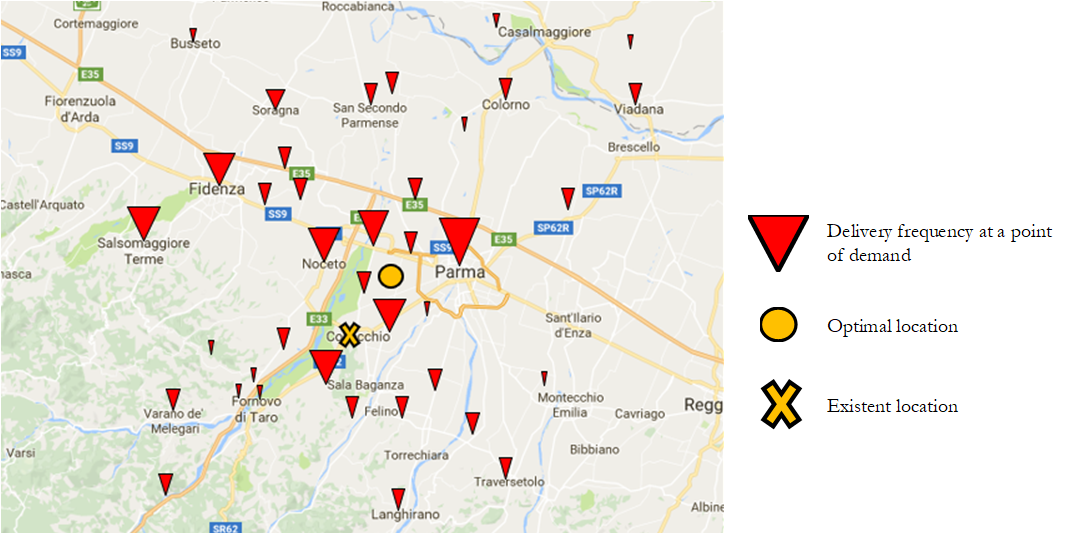
\includegraphics[width=0.9\textwidth]{sectionProduction/design_plant_figures/fig_prod_CAMST_ubicazione.png}
\captionsetup{type=figure}
\caption{Transition of the optimal location of the network considering different time periods.}
\label{fig_prod_CAMST_ubicazione}
\end{figure}

\subsubsection{Auxiliary systems design, technology and asset choice, definition of the number of assets and layout design}

Due to the peculiarity of the catering industry, a wide number of professionals with various competencies and backgrounds were involved in the design phase. To support the design of the new plant and to investigate how their decisions affect each other, a comprehensive decision support system (DSS) was developed ~\cite{Tufano2018_cekiDesign}. The DSS simulates the production operations by using a Montecarlo approach. Decision-makers can change the value of the decision levers regarding:

\begin{itemize}
    \item the auxiliary energy system to use (electricity, gas or steam);
    \item the type of asset to use;
    \item the number of assets for each type;
    \item the position of the control point where resources are placed.

\end{itemize}

The relational database illustrated in section \ref{secRelationalModelProduction} is the input dataset to feed the DSS. The DSS produces descriptive and visual analytics on the results of the simulation as, for example, the spaghetti chart (see Figure \ref{fig_prod_CAMST_spaghettiChart}), representing the intensity of the material flow exchanged between control points.

% INSERT fig_prod_CAMST_spaghettiChart
\begin{figure}[hbt!]
\centering
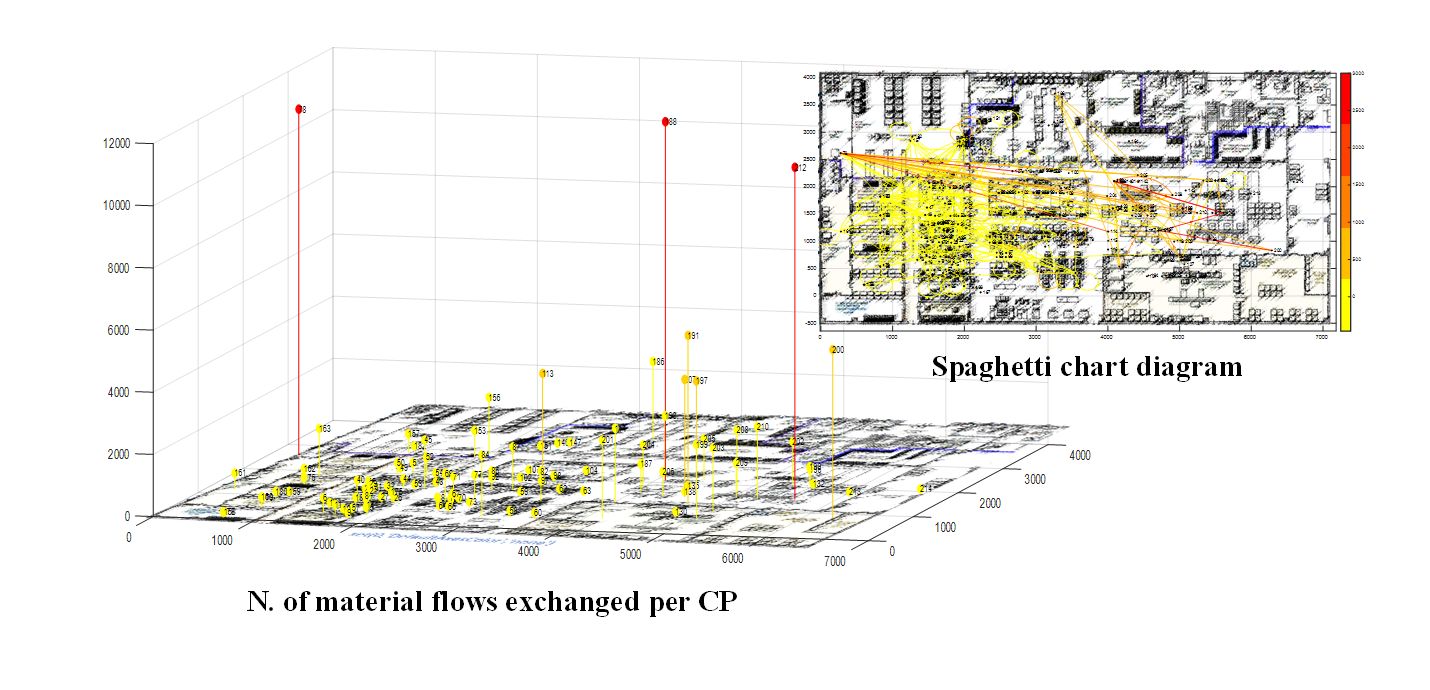
\includegraphics[width=0.9\textwidth]{sectionProduction/design_plant_figures/fig_prod_CAMST_spaghettiChart.png}
\captionsetup{type=figure}
\caption{Spaghetti chart and material flow intensity chart.}
\label{fig_prod_CAMST_spaghettiChart}
\end{figure}

Figure \ref{fig_prod_CAMST_workload} proposes insights about the effect of decision-making on the workload of the auxiliary systems for the production of energy and the workload of a single workstation (i.e. a machine). The two analytics look similar as they represent the expected utilization of the loading capacity of a generic working station and power load required by the plant (i.e., the electrical or thermal energy expressed in equivalent kWh of energy or gas) or gas loads over the timeline, respectively. The blue lines represent the utilization coefficient of a resource. This coefficient is calculated as the ratio between the volume of a product loaded on the resource to its loading capacity. A value of utilization less than unity indicates when a working station is underutilized, while values above unity indicate the theoretical number of resources needed to avoid queues.\par

The energy workload chart identifies the power load for different energy types, estimating the size and capacity of the power supply system. When different energy supplies are allowed for a given resource (i.e., trivalent oven), two alternative graphs are reported, and energy costs are quantified accordingly to assess the most convenient energy source.

% INSERT fig_prod_CAMST_workload
\begin{figure}[hbt!]
\centering
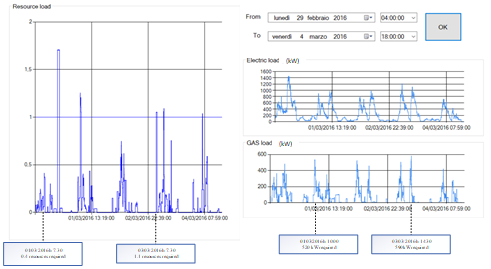
\includegraphics[width=0.9\textwidth]{sectionProduction/design_plant_figures/fig_prod_CAMST_workload.png}
\captionsetup{type=figure}
\caption{Representation of the workload and the energy profile of a set of different resources of the CEKI.}
\label{fig_prod_CAMST_workload}
\end{figure}

To investigate the behaviour of the system depending on the number of assets, the DSS implements three different rationales to identify the number of assets ~\cite{Tufano2019_bookChapterPlantDesign}. The simulation can be set up using:

\begin{itemize}
    \item a single machine for each type (machine-based rationale), to identify the workload curve of the machine;
    \item the minimum number of machine to avoid queues (recipe-based), to identify the behaviour of the system without queues;
    \item an arbitrary number of machine defined by the decision-maker (layout-based), to identify the performance of a given design alternative.

\end{itemize}

By using the DSS, managers can immediately investigate the logistic effect of their decisions. Additional information on the expected production time and costs are provided to identify which product may represent a bottleneck for the production system (see Figure \ref{fig_prod_CAMST_cost}).

% INSERT fig_prod_CAMST_cost
\begin{figure}[hbt!]
\centering
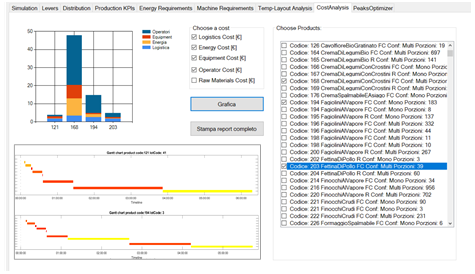
\includegraphics[width=0.9\textwidth]{sectionProduction/design_plant_figures/fig_prod_CAMST_cost.png}
\captionsetup{type=figure}
\caption{Dashboard identifying the cost and the schedule of each part processed by the CEKI.}
\label{fig_prod_CAMST_cost}
\end{figure}

The DSS allows them to develop many different production scenarios and to test their behaviour by using a simulation approach. This approach presents a high bias since it cannot be generalised to any production nodes. However, it gives the flexibility to the decision-makers of investigating how the decisions belonging to their specific field of responsibility (e.g. architectural, power plants, layout design, asset choice) modify the operational performance of the entire production system.

\subsection{Plant Design of a 3PL packaging plant for automotive spare parts}
This section illustrates the methodology to design a 3PL packaging plant for automotive spare parts from scratch.\par

The new plant is designed to replace an existing plant processing end-of-line tasks (e.g. picking, packing, placing, oiling, labelling) on more than 58.000 spare parts automotive supply chain. This type of processing plants works as an intermediate stage of the automotive supply chain where incoming products are collected, packaged and labelled according to the clients' needs. The clients are production plants where cars or tractors are assembled and prepared for shipping to the final user. Since these clients mainly work Just-In-Time (JIT), the 3PL packaging plant has to absorb an unpredictable demand in a very short time. \par

The plant delivers its service using three different due times (24, 48 and 72 hours) with an LoS of the 90\% (i.e. 90\% of the probability to deliver a service within the given LoS). The operations of the 3PL packaging plant consist of oiling, packing and labelling spare parts. \par

To properly design the new plant, it is necessary to assess the current state of the system and predict future demand as illustrated in \ref{secControlPackagingPlant}.

\subsubsection{Clustering products into families}

The first step for the design of the new production node is to define product families ~\cite{Tufano2020ISM}. As Figure 1 shows, the workload is highly variable. In addition, the quantity processed is variable too and slightly correlated with the number of lines processed. For these reasons, the definition of product families can help the design and control of the production systems. Since the production cycle is not available in the information system of the company, the idea is to cluster parts based on their feature, assuming the production cycle is similar. A correlation heatmap is built, considering the service type, the size, volume, weight and type of package of the items, to check this assumption. Figure \ref{fig_prod_CHIMAR_prodFamilies} shows a heatmap built on about two millions of orders for seven years.

% INSERT fig_prod_CHIMAR_prodFamilies
\begin{figure}[hbt!]
\centering
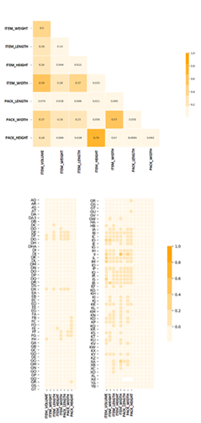
\includegraphics[width=0.7\textwidth]{sectionProduction/design_plant_figures/fig_prod_CHIMAR_prodFamilies.png}
\captionsetup{type=figure}
\caption{Correlation matrix of the features of the input dataset.}
\label{fig_prod_CHIMAR_prodFamilies}
\end{figure}

Figure \ref{fig_prod_CHIMAR_prodFamilies} reveals an obvious significant correlation between the dimensions of the package and the items. Besides, there are significant correlations between the dimensions of packages and items and some service type. This result suggests that there is the possibility to cluster item based on the service type and assign them to specific workbenches in order to reduce the complexity and the inventory of packages needed on each workbench.\par

Operators perform the tasks of a specific service type on manual workbenches with no automation. All the operators on the 12 workbenches can process any of the 58.000 products. This fact leads to a very low specialisation of the operators, and unpredictable material flows since any of the workbenches can request all the 1500 different types of packages. Besides, some clients require a customised tertiary package structured as a shelf of the dimension of a pallet. These shelves are placed directly to a workstation of the client’s assembly line. For this reason, the 3PL package plant has to deal with high work-in-process (WIP) levels on the workbenches due to products, packages (with the size of a carton box) and customised shelves (with the size of a pallet). To deal with this randomised material flows and WIP of the 3PL plants, we applied the proposed methodology aiming at the definition of a number of families. We start with an increasing number of cluster (from two to ten) using different clustering techniques (see section \ref{secClustering}). This value is, then, compared to an estimation of the real number of workbenches with the application of the capacitated clustering algorithm. Figure \ref{fig_prod_CHIMAR_clustering} presents the graphical results of the algorithms in the different clustering scenarios and with a different number of clusters. Each dot is one of the 58.000 products, while the axis of each subplot represents the first two principal components of the input dataset. Different colours indicate different product families. 

% INSERT fig_prod_CHIMAR_clustering
\begin{figure}[hbt!]
\centering
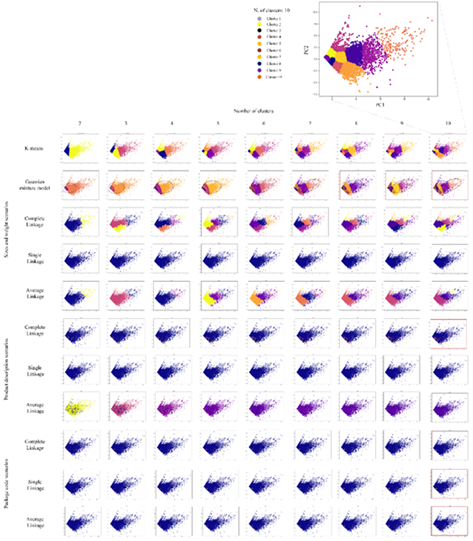
\includegraphics[width=0.9\textwidth]{sectionProduction/design_plant_figures/fig_prod_CHIMAR_clustering.png}
\captionsetup{type=figure}
\caption{Clustering of parts using different clustering algorithms, and different nuber of clusters.}
\label{fig_prod_CHIMAR_clustering}
\end{figure}

The output of unsupervised clustering is compared with the capacitated clustering algorithm (see algorithm \ref{algo_dist_CST}). The capacitated clustering algorithm considers a maximum allowable capacity that is fixed and equal for all the cluster and an amount of demand required by each product. To feed the algorithm with this data, we set a time and motion monitoring campaign in order to identify an average processing time required by each product. This data collection applied on a subset of the products (i.e. the items belonging to the 95\degree percentile of the total number of processed lines) due to the very high number of items. The amount of time required by the products with the highest workload defines the maximum capacity for each cluster. The capacitated clustering produces 20 clusters. This number is used to compare the performance with the best performing unsupervised models: the Gaussian Mixture Model and the Complete Linkage Clustering based on the Descriptions, setting the number of clusters $k=20$. \par

Figure \ref{fig_prod_CHIMAR_clusteringVisualisation} illustrates the outcome of this comparison using a visual analytics technique called t-SNE. This technique visually identifies clusters based on the matrix $X$, $n\times p$ of the observation that is projected onto a 2-dimensional space preserving the proximity of each observation according to the t-distribution. The colours are associated accordingly with the cluster assignment given by the algorithms. Figure \ref{fig_prod_CHIMAR_clusteringVisualisation} shows that it is difficult to identify a topology of the cluster (as it happens in Figure \ref{fig_prod_CHIMAR_clustering}) since the number of clusters is high and the input data are scattered. On the other side, analysing Table \ref{tab_prod_CHIMAR_familiesPerformance} it is possible to evaluate the performance of the algorithm from a logistic point of view, identifying the variability of the processes organised according to this clustering. 

% INSERT fig_prod_CHIMAR_clusteringVisualisation
\begin{figure}[hbt!]
\centering
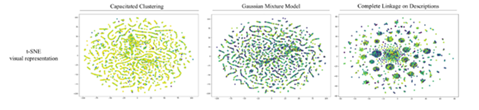
\includegraphics[width=0.9\textwidth]{sectionProduction/design_plant_figures/fig_prod_CHIMAR_clusteringVisualisation.png}
\captionsetup{type=figure}
\caption{Comparison of the topology of the cluster using the t-sne algorithm. Colors identifies parts belonging to the same cluster.}
\label{fig_prod_CHIMAR_clusteringVisualisation}
\end{figure}

Table \ref{tab_prod_CHIMAR_familiesPerformance} illustrates the KPIs and compares their variance (using absolute and relative value compared to the capacitated case) calculated on a time horizon of 7 years. It is easy to check that the capacitated clustering provides the highest balanced scenario with the lowest variance. The variance in workload (i.e. seconds) between the 20 clusters has an average of 180 hours per year per workbenches. This is a low gap, considering that the variability in the number of products and packages is dramatically reduced compared to the other scenarios.

% INSERT tab_prod_CHIMAR_familiesPerformance
\begin{figure}[hbt!]
\centering
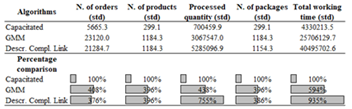
\includegraphics[width=0.9\textwidth]{sectionProduction/design_plant_figures/tab_prod_CHIMAR_familiesPerformance.png}
\captionsetup{type=table}
\caption{Comparison of the logistic impact between capacitated and uncapacitated algorithms.}
\label{tab_prod_CHIMAR_familiesPerformance}
\end{figure}

Gaussian Mixture Model provides a poorer result that has to be manually checked and assessed before a physical implementation since a couple of clusters results extremely small in workload compared to the average of the others. Nevertheless, it is important to remember that GMM provides the uncapacitated result in short running time (i.e. about 5 minutes) compared to a long runtime of the capacitated algorithm which needs around 20 hours of runtime on a computer equipped with 8Gb memory and a 2.7GHz processor. 

\subsubsection{Facility location}
Facility location has been studied by using a probabilistic approach, identifying for each year of the input dataset the optimal location in three different scenarios. The scenarios are defined by the distance metrics, i.e. euclidean, rectangular and squared euclidean distance. Figure \ref{fig_prod_CHIMAR_location} identifies the results on the map where each row is a different distance scenario, and each column identifies how the optimal location – according to the chosen distance – moves on the map. The bubbles identify the intensity of the yearly aggregated flows exchanged with suppliers and customers.\footnote{The source code of Figure \ref{fig_prod_CHIMAR_location} is available \href{https://github.com/aletuf93/logproj/blob/master/examples/PROD_01\%20Facility\%20location.ipynb}{here}.}

% INSERT fig_prod_CHIMAR_location
\begin{figure}[hbt!]
\centering
\includegraphics[width=0.9\textwidth]{sectionProduction/design_plant_figures/fig_prod_CHIMAR_location.png}
\captionsetup{type=figure}
\caption{Comparison of the optimal location produced using different distance metric (i.e. euclidean, rectangular, and gravity) and different time periods.}
\label{fig_prod_CHIMAR_location}
\end{figure}







\clearpage
\bibliographystyle{ieeetr}
\bibliography{sectionProduction/design_plant_ref}